\documentclass[11pt, us-letter]{article}
\usepackage{times}
\usepackage{graphicx}
\usepackage{wrapfig}
\usepackage{color}
\usepackage{xspace}
\usepackage{url}
\usepackage{subfigure}
\usepackage{algorithm2e}
\usepackage[letterpaper, top=.9in, bottom=.9in, inner=.9in, outer=.9in, foot=.25in]{geometry}
\usepackage{amsmath,amsfonts,amsthm,amssymb}
\usepackage{array}
\usepackage{listings}
\usepackage{comment}

\usepackage[compact]{titlesec}
\titlespacing{\section}{0pt}{6pt}{4pt}
\titlespacing{\subsection}{0pt}{5pt}{3pt}
\titlespacing{\subsubsection}{0pt}{5pt}{3pt}


\newcommand{\mytitle}{BIGDATA:Small:Data Collection and Management:\\Widespread CALM: Coordination Analysis and Big Data}

\newcommand{\denselist}{
\addtolength{\itemsep}{-7pt}}
%\setlength{\listparindent}{-170pt}}
%\addtolength{\partopsep}{-40pt}}

%\addtolength{\textwidth}{10mm}
%\addtolength{\textheight}{10mm}
\renewcommand{\baselinestretch}{0.95}

\renewcommand{\paragraph}[1]{\vspace*{2mm}\noindent\textbf{#1} \ \ }

% FORMATTING -------------------------------------------------------
\newcommand{\term}[1]{\textbf{#1}}
\newcommand{\figref}[1]{Figure~\ref{#1}}
\newcommand{\secref}[1]{Section~\ref{#1}}
\newcommand{\eqnref}[1]{Equation~\ref{#1}}
\newcolumntype{C}[1]{>{\centering\arraybackslash}p{#1}}
\newcommand{\itembf}[1]{\item\textbf{#1}}
\newenvironment{tightitemize}{\begin{list}{$\bullet$}{\setlength{\itemsep}{1pt}\setlength{\topsep}{2pt}\setlength{\parskip}{1pt}\setlength{\parsep}{1pt}\leftmargin=1.5em}}{\end{list}}


% THEOREMS -------------------------------------------------------
\newtheorem{thm}{Theorem}[section]
\newtheorem{cor}{Corollary}
\newtheorem{lem}{Lemma}
\newtheorem{prop}{Proposition}
%\theoremstyle{definition}
\newtheorem{defn}{Definition}
\newtheorem{property}{Property}
%\theoremstyle{remark}
\newtheorem{rem}{Remark}
%\theoremstyle{assumption}
\newtheorem{assumpt}{Assumption}
%\numberwithin{equation}{section}
\newtheorem{example}{Example}
\newtheorem{ex}[thm]{Example}
\newtheorem{exa}{Example}
\newtheorem{dfn}{Definition}[section]
\newtheorem{goal}{Goal}


% inline comments
% color names at http://en.wikibooks.org/wiki/LaTeX/Colors#Predefined_colors
\usepackage[usenames,dvipsnames]{xcolor}
\newcommand{\jmh}[1]{{\textcolor{red}{#1 -- jmh}}}

% indent full paragraph for compact lists
\newenvironment{myparindent} {
  \hangindent=1em
  \hangafter=0
  \noindent
}

%captionsmall -- format captions in a smaller font
\newcommand{\captionsmall}[1]{\caption{\footnotesize{#1}}}

% Comment out to take away comments
\newcommand{\commentout}[1]{}
\newcommand{\out}[1]{}

% no page numbers
%\pagestyle{empty}


\newcommand{\myurl}[1]{{\footnotesize \url{#1}}}
\def\blooml{Bloom$^L$\xspace}

\begin{document}

\usepackage{color}
\usepackage{graphicx}
\usepackage{url}
\usepackage{xspace}
\usepackage[T1]{fontenc}
\usepackage{times}
%\usepackage{mathptmx}    % use "times" font, including for math mode
\usepackage{txfonts}  % apparently needed to fixup the formatting of lstlistings
\usepackage{textcomp}
\usepackage[protrusion=true,expansion=true]{microtype}
\usepackage{paralist}
\usepackage{comment}
%\usepackage[hidelinks]{hyperref}

\def\blooml{Bloom$^L$\xspace}

\frenchspacing

\begin{document}

\title{Distributed Programming and Consistency:\\Principles and Practice}

\numberofauthors{3}
\author{
\alignauthor
Peter Alvaro\\
        \affaddr{UC Berkeley}\\
        \email{palvaro@cs.berkeley.edu}
\alignauthor
Neil Conway\\
        \affaddr{UC Berkeley}\\
        \email{nrc@cs.berkeley.edu}
\alignauthor
Joseph M.\ Hellerstein\\
        \affaddr{UC Berkeley}\\
        \email{hellerstein@cs.berkeley.edu}
}

\maketitle

\section{Introduction}

In recent years, distributed programming has become a topic of widespread
interest among developers. However, writing reliable distributed programs
remains stubbornly difficult. In addition to the inherent challenges of
distribution---asynchrony, concurrency, and partial failure---many modern
distributed systems operate at massive scale. Scalability concerns have in turn
encouraged many developers to eschew strongly consistent distributed storage in
favor of application-level consistency criteria~\cite{Birman2009,Helland2009,vogels},
which has raised the degree of difficulty still further.

To cope with the challenges of distributed programming without the benefit of
strong consistency, practitioners have developed rules of thumb, such as using
commutative, associative, and idempotent operations when
possible~\cite{Helland2009,Pritchett2008} and employing application semantics to
resolve divergent replica states~\cite{DeCandia2007}. However, until recently
there was relatively little work on principled approaches to enable
application-level consistency criteria without requiring global coordination.

In this tutorial, we will review recent research on principled approaches to
eventually consistent
programming~\cite{Alvaro2011,Burckhardt2012,Conway2012,Hellerstein2010,Roh2011,Shapiro2011a,Shapiro2011b},
and connect this body of work to practical systems and design patterns used by
practitioners. We will begin by discussing how \emph{semilattices} can be used to
reason about the convergence of replicated data values, following the ``CRDT''
framework recently proposed by Shapiro et
al.~\cite{Shapiro2011a,Shapiro2011b}. After presenting several examples of how
lattices can be used to achieve consistency without coordination, we will then
discuss how lattices can be composed using \emph{monotone functions} to form
more complex applications~\cite{Conway2012}. We will connect this work to the tradition of logic programming from the database community~\cite{AliceBook}, and to our work on the
\emph{CALM Theorem}, which characterizes the need for distributed coordination to 
ensure consistency at application level~\cite{Alvaro2011,Ameloot2011,Hellerstein2010,dedalus-confluence}. 

\begin{comment}
Finally,
we will discuss several design options for supporting non-monotonic operations:
\begin{compactenum}[(a)]
\item introducing coordination at appropriate program locations identified by
  CALM analysis
\item employing ``weak coordination'' as a background operation (e.g., for distributed
garbage collection)
\item tolerating and then correcting inconsistency using taint tracking and
after-the-fact ``apology'' or compensation logic~\cite{Garcia-Molina1987,Helland2009,Korth1990}
\end{compactenum}
We will conclude by summarizing the state of the art and highlighting open
problems and challenges in the field.
\end{comment}

Throughout the tutorial, we will use \emph{Bloom}, a language for distributed
programming that we have developed at Berkeley~\cite{bloom-website}. We will
demonstrate the concepts introduced in this tutorial by using Bloom to interactively 
develop well-known distributed systems infrastructure components, including a key-value
store, quorum replication, a distributed lock manager with deadlock detection,
and a distributed commit protocol. Using tools distributed with the Bloom
runtime, we will show how developers can visualize the distributed behavior of
their programs, reason about the need for coordination across software components, compose
individual monotonic components into larger programs, and employ Bloom's
built-in tools for systematic distributed testing~\cite{Alvaro2012}.

The tutorial will be \emph{interactive}, in that installation instructions for
the Bloom runtime will be provided and attendees will be given the complete
source code for all example programs. During the tutorial, we plan to use the
Bloom runtime to execute example programs, use the the built-in Bloom analysis
tools to understand program behavior, and iteratively refine programs as
appropriate. Attendees will have the option to run the tools themselves,
although participation int this manner will not be mandatory. Note that for time
reasons we do not expect attendees to develop Bloom programs from scratch during
the tutorial, although several ``homework'' assignments will be made available
to extend the example programs we present.

\section{Objectives and Outcomes}

\begin{enumerate}
\item
  Discuss the particular challenges and benefits associated with programming
  over systems that provide only eventual
  consistency~\cite{DeCandia2007,Terry1995,vogels}, rather than the stronger
  guarantees provided by traditional distributed transactional systems.
  Summarize the motivations behind the current trend away from widespread use of
  strong consistency protocols at scale.
\item
  Introduce and compare recent research proposals to simplify distributed
  programming without strong consistency.  Present abstract design patterns
  for working with eventually consistent systems.
\item
  Focus on the CRDT and CALM approaches to distributed consistency, and show how
  lattices and monotone functions can be used to build provably convergent
  implementations of well-known distributed infrastructure.  Provide concrete
  examples of CvRDTs including sets, counters, and graphs, and illustrate how
  these data structures achieve eventual consistency.
\item
  Discuss the CALM Theorem, which sheds light on \emph{why} certain programs
  require distributed coordination and why others do not.  Characterize the
  situations in which monotone programs are not sufficient, and discuss several
  ways in which non-monotonic operations can be supported.
\item
  Introduce the Bloom programming language and related tools for visualization,
  debugging, and systematic testing of distributed programs.
\item
  As a running example, implement a family of key-value store designs with
  various consistency guarantees in Bloom.  Aided by static analysis tools,
  contrast the nondeterministic executions of overwrite-based stores with stores
  whose values are constrained to be lattices, and hence are convergent in
  either the value or version domain.  Illustrate the use of lattice
  compositions to implement quorum replication, which can be parameterized to
  enforce strong or eventual consistency.
\item
  Nonmonotonicity cannot always be avoided.  Discuss recent and future work on mitigating
the problems that can arise in nonmonotonic distributed systems.  Show how CALM analysis
can be used to identify program locations at which coordination can be added by the programmer
or synthesized by the runtime.  Discuss approached that tolelated and attempt to correct
inconsistencies using delayed coordination, compensatory actions or ``apologies.''  
Present constructive strategies
for ``sealing'' (or making immutable) certain partitions of the program input, to prevent
subsequent nonmontonic operations from producing inconsistent states.

\item
  Highlight open problems and research challenges in the area of principled
  eventual consistency.
\end{enumerate}


\bibliographystyle{abbrv}
\bibliography{summary}

\end{document}


\pagebreak

\section{Introduction}
\label{sec:intro}
\section{Introduction} 
\label{sec:intro} 
Although distributed programming has become an essential and commonplace task,
it remains very challenging for most developers to write correct distributed
programs. The inherent difficulties of distributed computing---concurrency,
asynchrony, and partial failure---are exacerbated by the scale at which modern
distributed systems operate.

% remind reviewers that it's a database problem. can remove if accepted! 
Much of the discussion about distributed programming today revolves around data
management systems, and the tradeoffs between transactions and loose
consistency. Programmers using distributed transactions are relieved of
consistency concerns but often face significant performance and operational
challenges~\cite{Birman2009}. By contrast, programmers who use loosely
consistent systems can expect more predictable and low-latency performance, but
must reason explicitly about program correctness over inconsistent distributed
state.

In recent years there has been increased interest in techniques to help
programmers achieve correct program behavior without requiring strongly
consistent storage. This idea has been explored in two different frameworks,
\emph{Convergent Objects} and \emph{Monotonic Logic}.

\vspace{0.5em}\noindent
\textbf{Convergent Objects}: In this approach, a programmer writes encapsulated
object classes whose public methods guarantee certain properties regarding
message reordering and/or retry. For example, Statebox is an open-source library
that merges conflicting updates to data items in a key-value store; the user of
the library need only register commutative, idempotent merge
functions~\cite{statebox}. This approach has roots in research in
databases~\cite{Farrag1989,Garcia-Molina1983,Helland2009} and
groupware~\cite{Ellis1989,Sun1998}.  Shapiro et al.\ recently proposed a model
for these approaches called \emph{Conflict-Free Replicated Data Types} (CRDTs),
which formalizes these ideas in an algebraic framework~\cite{Shapiro2011b}.

The main problem with the CRDT approach is that its guarantees of correctness
are limited to an individual replicated data value, not to application logic in
general. For example, consider a distributed algorithmic trading service that
uses a CRDT to represent a mutable set \texttt{Portfolio}. Suppose one server
$M$ reads a local version of the set containing an element \texttt{BNNA} and
constructs an expected portfolio value $v = f(\mbox{\texttt{Portfolio}})$
derived from that version. Concurrently, \texttt{BNNA} is removed from the local
version of \texttt{Portfolio} at another server $N$. The CRDT can ensure that
$M$ and $N$ will eventually agree that \texttt{BNNA} is absent from the set, but
the application state at $M$ and $N$ may remain inconsistent unless the value
$v$ at $M$ is updated to reflect the removal of \texttt{BNNA}. Although the CRDT
maintains its own invariants, the programmer still bears the burden of ensuring
the consistency semantics of the entire program.

\vspace{0.5em} \noindent
\textbf{Monotonic Logic}: In recent work, we observed that the database theory
literature on non-monotonic logic provides a promising starting point for
reasoning about distributed consistency. Intuitively, a \emph{monotonic} program
computes more information over time---it never ``retracts'' an earlier
conclusion in the face of new information. We proposed the CALM
theorem~\cite{Hellerstein2010}, which established that all monotonic programs
are eventually consistent~\cite{Ameloot2011,dedalus-pods12-tr}. Monotonicity of
a Datalog-style program is straightforward to determine conservatively from
syntax, so the CALM theorem provides the basis for a simple analysis technique
for verifying the consistency of distributed programs~\cite{Alvaro2011}. We
realized the CALM analysis as part of Bloom, a Datalog-based DSL for distributed
programming~\cite{bloom}.

The original formulation of Bloom and CALM only validated consistency for programs that compute sets of facts that grow over time (``set monotonicity''); that is, ``growth'' is defined according to set containment. As a practical matter, this is overly conservative: several common distributed programming idioms that are monotonic do not satisfy syntactic monotonicity tests for Datalog. In particular, threshold tests over monotonic aggregate values (e.g., ``$\mathrm{max}(S) > k$'') and upward-moving mutable counters are both considered to be non-monotonic by the original CALM analysis.  As a result, the initial Bloom prototype advises the programmer to guard those constructs with strong consistency methods like Paxos~\cite{Lamport1998} or Two-Phase Commit. 

\subsection{A Hybrid Approach}
% The strengths and weaknesses of these two approaches appear complementary. CRDTs provide synchronization-free consistent objects, but cannot guarantee whole-program consistency. Bloom's CALM analysis guarantees whole-program consistency but is unable to verify a number of natural coordination-free mechanisms.
In this paper, we extend our previous work to accommodate the ideas underlying CRDTs. Instead of only allowing growth according to the set containment
partial order, we allow any user-defined partial order to be used.  
We do this by providing \emph{join semi-lattices} as a programming construct.
We give a
formal definition of this construct below, but the intuition is that the programmer provides a commutative, idempotent merge function (``least upper bound'')
that takes two input values and produces an output value that is not smaller
than either of the input values (according to the user's partial order). This
generalizes Bloom (and traditional Datalog), which assumes a fixed merge
function (set union) and partial order (set containment).
% Relate user-defined merge functions to merge functions in other contexts?
% (e.g., key-value store, COPS, Piccolo)

% Explain how lattices generalize monotonic datalog
It is attractive to incorporate join semi-lattices into logic programming,  but doing so raises challenges in language design, consistency analysis and efficient execution.  In this paper, we make the following contributions:
\begin{enumerate}
% \item
%   We present \baselang, a variant of Datalog that is defined over lattices. We
%   define a model-theoretic semantics for \baselang, and show that \baselang
%   generalizes Datalog.

\item
  We introduce \lang, an extension of Bloom that supports lattices. We detail
  the builtin lattice types provided by \lang and show how developers can
  define new lattices.
  
\item 
  We provide interfaces for consistency-preserving mappings across lattices via
  \emph{morphisms} and \emph{monotonic functions}.  This is critical for \lang
  and forms a useful extension to the CRDT framework as well.

\item 
  We generalize the CALM analysis to programs that contain both lattices and
  set-oriented collections, and show how lattices can be used to prove the
  confluence of several common distributed design patterns that were regarded as
  non-monotonic in Bloom. % XXX: revisit this

\item
  For efficient execution, we show how to extend the standard Datalog semi-naive
  evaluation scheme~\cite{Balbin1987} to support both lattices and traditional
  database relations. We also describe how an existing Datalog engine can be
  extended to support lattices with relatively minor changes.

\item
  Finally, we demonstrate the usefulness of lattices with two case studies.
  First we revisit the simple e-commerce scenario presented in Alvaro et al., in
  which clients interact with a replicated shopping cart
  service~\cite{Alvaro2011}. We show how \lang can be used to make the
  ``checkout'' operation monotonic, despite the fact that it requires
  aggregating over a distributed data set.

  Second, we use \lang to implement vector clocks and causal delivery, two
  standard building blocks for distributed programming. We show how both
  algorithms can be realized as monotonic \lang programs that are concise and
  readable.
\end{enumerate}


\section{CALM Beyond Sets}
\label{sec:lattice}
%!TEX root = proposal.tex
To achieve consistency without using expensive distributed coordination, many
systems have proposed using a vocabulary of \emph{commutative} operations
(e.g.,~\cite{dynamo,Reiher1994,bayou}); this allows the replicas of a distributed
object to process events in different orders and converge to the same final
state. This approach has recently been formalized 

\jmh{Intro paragraph.}
\begin{itemize}
\item Crib motivation from VLDB submission, shortening the CRDT and Bloom background and moving straight to the idea of solving the type dilemma (as discussed in Intro) by merging them. (Cite Ross/Sagiv along the way.)
\item Discuss the idea of extending Bloom logic programming and CALM analysis to disorderly programs over arbitrary lattices. Say we've got an initial prototype of BloomL -- can cite TR if we like.
\item Give an example of a Bloom rule over sets and a corresponding rule over lmaxes.  
\item Discuss mappings, commutative functions and homomorphisms.  Impact on CALM and delta computation.
\item Show the vector clock example in a box.
\item Challenge: proving lattice properties. Possible conservative analysis in a nice imperative language, or a subsetted DSL within such a language., 
\item Challenge: Lattices and efficiency: garbage collection and lower bounds
\item Challenge: Lattices and non-monotonicity: e.g. ``odometer'' compositions, etc.
\end{itemize}

\subsection{Summary of Tasks and Goals}
\begin{itemize}
\item \textbf{Efficient Evaluation of Lattice programs}.  \jmh{Sentence or 2 here on Lower bounds, zero-copy, etc.}
\item \textbf{Tools for guaranteed lattice properties}.  \jmh{Sentence or two here on a possible DSL agenda, perhaps subsetting some existing language like Scala.  Remind that scope can be small because so much can be done outside the DSL in BloomL via lattice composition (e.g. data structures).}
\item \textbf{Extend the Bloom prototype to support rich set of built-in for composition.}  \jmh{Sentence or two here on what's involved, including language design and evaluation.  Say we've got a first prototype, and highlight remaining challenges.}.
\item \textbf{Evaluations: KVSs and Collaborative Editors.}  \jmh{Sentence or two here pitching the challenge here, and sketching some milestones/metrics for success}.
\end{itemize}

\section{CALM Service Composition}
\label{sec:soa}
%!TEX root = proposal.tex

Our static analysis techniques for Bloom can
%conservatively 
affirm that a given program has eventually consistent outcomes.
If the analysis is unable to do so---due to the presence of non-monotonic deductions
that follow asynchronous communication---a dataflow visualization tool can display the
program locations where coordination may need to be added to ``guard'' the
non-monotonic operations.  
Figure~\ref{fig:kvs} shows a Bloom implementation of a simple key-value store
and its accompanying dataflow visualization.  Note the white circles on the edges leading
into the \texttt{kvstate} collection, indicating non-monotonic operations corresponding to 
the deletion in lines~\ref{line:bloom-kvs-del1} and~\ref{line:bloom-kvs-del2}; clicking on those circles brings up the relevant non-monotonic statements.


\begin{figure}[t]
\begin{minipage}{.48\textwidth}

\begin{scriptsize}
\begin{lstlisting}
module KVSProtocol
  state do
    interface input, :kvput, [:client, :key] => [:reqid, :value]
    interface input, :kvdel, [:key] => [:reqid]
    interface input, :kvget, [:reqid] => [:key]
    interface output, :kvget_response, [:reqid] => [:key, :value]
  end
end

module BasicKVS
  include KVSProtocol

  state do
    table :kvstate, [:key] => [:value]
  end

  bloom :mutate do
    kvstate <+ kvput {|s| [s.key, s.value]}
    kvstate <- (kvstate * kvput).lefts(:key => :key) (*\label{line:bloom-kvs-del1}*)
    kvstate <- (kvstate * kvdel).lefts(:key => :key) (*\label{line:bloom-kvs-del2}*)
  end

  bloom :get do
    temp :getj <= (kvget * kvstate).pairs(:key => :key)
    kvget_response <= getj do |g, t|
      [g.reqid, t.key, t.value]
    end
  end

end

\end{lstlisting}
\end{scriptsize}
\end{minipage}
\begin{minipage}{.48\textwidth}
\raggedleft
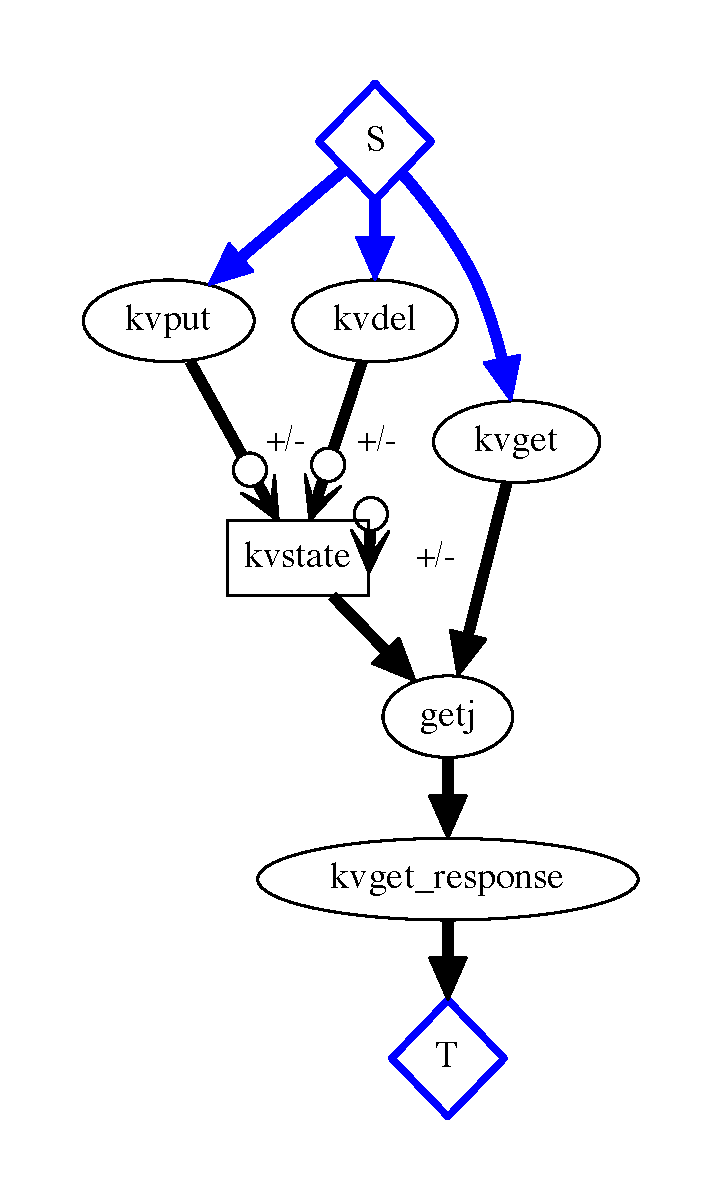
\includegraphics[width=0.7\linewidth]{kvs.pdf}
\end{minipage}

\vspace{-10pt}
\caption{A Bloom key-value store and its CALM visualization}
\label{fig:kvs}
\vspace{-2pt}

\end{figure}

The interface presents a visualization of the static dataflow analysis that we perform on a Bloom program.  While useful, such visualizations do not scale well to large programs and big graphs. Moreover, in many cases a programmer does not want to see this level of detail for all the code in their program.  For instance, when using encapsulated library modules, it is helpful to reason only about their interfaces, not their internals.  Ideally, CALM analysis should be encapsulated via annotations on a module's external input/output API, exposing only the consistency implications of composing the module with other code.

\begin{figure}[t]
\begin{minipage}{.63\textwidth}
\footnotesize

%%\centering
\begin{tabular}{|l|l|p{7cm}|}
\hline
Class & Label & Interpretation \\ \hline
Primitive & $\bot$ & Transformation does not affect consistency \\ \cline{2-3}
& $N$ & Non-monotonic (order-sensitive) transformation \\ \cline{2-3}
& $A$ & Asynchronous (unordered) communication \\ \hline
Compound & $D$ & Diffluent (non-confluent): non-deterministic results across executions or replicas \\ \cline{2-3}
& $R$ & Restores order.  Represents some coordination protocol. \\ \hline

\end{tabular}

%\vspace{-10pt}
%\caption{Consistency Labels}
%\label{fig:basic-labels}
%\vspace{-2pt}
%\end{figure}


%\begin{figure}[t]

\end{minipage}
\begin{minipage}{.35\textwidth}
\raggedleft

\footnotesize
\begin{tabular}{|l|p{4cm}|}
\hline
Rule & Interpretation \\ \hline
$\alpha\alpha \rightarrow \alpha$ & label repetition does not change semantics \\ \hline
$\bot \beta \rightarrow \beta$ & $\bot$ has no effect on neighboring \\
$\beta \bot \rightarrow \beta$ & labels\\ \hline
$AN \rightarrow D$ & Loss of order followed by order-sensitivity causes diffluence \\ \hline
$D \alpha \rightarrow D$ & \\
$\alpha D \rightarrow D$ & Once diffluent, always diffluent\\ \hline
$AR \rightarrow R$ & Order lost and regained \\ \hline
$RA \rightarrow A$ & Order imposed and then lost \\ \hline
$RN \rightarrow R$ & $N$ does no harm to $R$ flows \\ \hline
$NR \rightarrow N$ & $R$ does no good for $N$ flows \\ \hline

\end{tabular}
\end{minipage}
\caption{Labels and Reduction Rules \jmh{what is the distinction between $\alpha$ and $\beta$ and did I use them right?}}
\label{fig:rules}
\end{figure}

To summarize the input-to-output relationships in a module, we have to characterize the dataflow \emph{paths} from each of its input interfaces to each of its output interfaces.  We do this by (1) labeling individual edges of a dataflow graph like Figure~\ref{fig:kvs} with key properties, and (2) understanding the transitive implications of these properties across multiple edges.  The left side of Figure~\ref{fig:rules} shows the labels that the analysis assigns to individual edges (``primitive''), and the labels that arise via dataflow composition (``compound'') as described in the rules on the right side of Figure~\ref{fig:rules}.  

As an illustration, consider again the overwriting key-value store presented in Figure~\ref{fig:kvs}.
CALM analysis detected a non-monotonic operation in the dataflow edge from \texttt{kvput} to \texttt{kvstate}: the appearance of PUT requests contribute to the deletion of old values (line~\ref{line:bloom-kvs-del1}).  Thus we label that edge with an $N$.  The other edge labels in Figure~\ref{fig:kvs} are either $N$ or $\bot$, so as we transitively combine edges, the first two rules on the right side of Figure~\ref{fig:rules} lead us to associate with BasicKVS the following signature for the single output interface and two input interfaces:
$kvget\_response: \{N(put) \; | \; \bot(get)\}$.  

Consider now a larger system that uses this key-value store as a component.  It will not be safe to attach an asynchronous ($A$)
stream to the \texttt{kvput} interface of the store, as this will lead to a divergent consistency label
(due to the rule $AN \rightarrow D$).  For asynchronous ($A$) inputs to this module,
order must be \emph{restored} (via
interposition of a dataflow labeled $R$) 
before composing with \texttt{kvput}.  This corresponds to intuition:
a key-value store with ``last writer wins'' semantics like Figure~\ref{fig:kvs} is clearly sensitive to the order in which it receives writes.
If the KVS is replicated, we must be careful about write reordering in the network, as this
may lead to inconsistent state on different replicas.
Reads, on the other hand, may be reordered freely.

\subsection{Widespread CALM Analysis: Service Composition}
The analysis framework above is helpful for analyzing pure Bloom programs that span multiple modules.
In practice, however, many distributed applications are not written in any single language, nor are all their components available for deep analysis.  Instead, many systems are compositions of large distributed services, loosely coupled using message-based APIs.
Such services are often implemented in a variety of programming 
languages, and in some cases they are opaque and outside the control of
the programmer using them.  
Many services (e.g. data stores and message queues) provide their own 
consistency guarantees, but how are we to reason about the consistency of an end-to-end
\emph{application} that calls out to various such services and transforms
and combines their responses?  

% We believe that the intuitions behind the CALM Theorem should apply at this level of reasoning,
% just as they applied to the low-level composition of operators
% in a Bloom execution.  We envision a scenario where Bloom is used as an \emph{orchestration} language for composing applications from multiple services.  The ``primitive'' consistency properties of many services in wide use today are well-known: for example, there are various libraries for distributed consensus that could be labeled $R$, there are various libraries for order-insensitive key-value stores that could be labeled $\bot$, and so on.  

% Consider an inventory management application 
% that makes calls into two asynchronously updated but
% eventually consistent datastores.  It selects from the first service---an 
% inventory datastore---the model numbers of all toaster ovens that are currently in stock.  For each, it probes the second datastore---a recall database---to
% see if the unit has been recalled.  Finally, the application returns the 
% set of model numbers for units that have \emph{not} been recalled.  Observe that this
% application has a race condition due to the negation (``not recalled''): for a given model number $N$, the order of a request to lookup $N$ and a request to insert a recall for $N$ will determine whether or not the system returns $N$.  In a distributed implementation, both orderings could occur at different replicas, yielding inconsistent results.  
% If the orchestration
% application that correlates the results from the different datastores were written in Bloom, we would observe that although the datastores are monotonic, 
% the manner in which their results are \emph{used} is not.  If the inputs to 
% the datastores are asynchronous (reorderable), then the output of the 
% application may be inconsistent.  In the Bloom labeling system presented above, both services would be labeled 
% $A$---that is, asynchronously updated but otherwise monotonic.  The orchestration code that connects them would be 
% labeled $N$---non-monotonic, due to the negation.  The resulting composition would then be labeled $D$---divergent, with
% a point of order in the orchestration code that should be resolved (e.g., by versioning the recall database and issuing queries against the 
% oldest ``complete'' version).
% 
% 
% \jmh{Make an explicit plan here to do something new with widely used systems -- zookeeper+voldemort+something?  Perhaps talk about potential collaboration with LinkedIn.}

The labeling system presented above provides a framework for reasoning about service composition that is 
mostly independent of Bloom, so long as we can accurately attribute consistency labels to service APIs.
If the services are written in Bloom, we can derive their labels automatically---otherwise we may rely on annotations.
As the example above indicated, however, we must be very careful how we \emph{use} data returned from 
eventually consistent services
if we wish to assert that application output is likewise consistent.  Hence the ``glue'' language used
to compose services must also be amenable to CALM analysis and label propagation.

\subsection{Summary of Tasks and Goals}
\begin{itemize}
\item \textbf{Path labeling and label propagation}.
The framework of labels and rules in Figure~\ref{fig:rules} is not yet complete; we are still formalizing its theory to prove correctness, and developing the program analysis tools to automatically label code written in Bloom and \blooml.  The labeling technique should be a confluent term rewriting system, allowing us to 
characterize any dataflow as a compact expression with an intuitive 
meaning in the context of distributed systems.

\item \textbf{Automated coordination synthesis}.
For inconsistent (diffluent) programs, we want to enhance them with order-restoring coordination mechanisms ($R$) to achieve consistency.
Programmers can supply their own coordination protocols, but we also hope that CALM analysis can lead to automatic synthesis of coordination code. 
It seems clear that a generic coordination 
protocol (e.g., totally ordered broadcast) may be interposed at arbitrary 
``points of order''
to ensure consistency.  More interestingly, we would like to automatically
discover cases where more efficient but more limited protocols---e.g., totally ordered unicast between pairs of nodes---are sufficient to ensure consistency.  We could then search the space of points-of-order and coordination protocols and (semi-)automatically choose the most efficient way to convert a disorderly and inconsistent program into a judiciously-ordered consistent program.

\item \textbf{Uniform error communication and handling}.
A significant challenge for an orchestration language is to provide robust error handling.
Calls to services can fail in various ways; in some cases services can report the error
back to the caller along with relevant information about its cause, while in other cases
applications must manage timeout and retry logic.  Since a robust orchestration language will
be fundamentally non-deterministic, we will have to revisit the consistency labeling system to
accommodate this uncertainty.

\item \textbf{Evaluation}.  As a proof of concept, we intend to implement a collection of services and applications for a social network setting implemented via a Service-Oriented Architecture.  We currently are collaborating with engineers at LinkedIn and plan to either emulate or integrate with their architecture, which is based heavily on open-source services.
We hope to show how CALM analysis can ease the burden of reasoning about the behavior of applications
that call out to a number of services (including data stores, message queues, coordination services like Zookeeper, 
and logging subsystems)
with various service-level consistency guarantees.

\end{itemize}



\section{CALM over Distributed Storage}
\label{sec:storage}
%!TEX root = proposal.tex
In many systems, distributed storage is a built-in construct, providing read and write facilities that offer transparency with respect to the physical location of data.  Because storage is a distributed subsystem, there is inherent asynchrony that is implicit in its implementation, which  entails built-in choices regarding consistency guarantees. Traditional distributed and parallel databases ensure serializability at the expense of coordination during commit processing.  By contrast, distributed filesystems and ``NoSQL'' key-value stores often provide some flavor of eventual consistency.  We have studied currently-popular eventually-consistent storage systems in our group in significant detail~\cite{boomanalytics,bailis}.

Bloom was originally designed as a flexible distributed systems language that makes no assumptions along these lines.  We considered it important that the  programmer of a distributed system maintain control over both the semantics of distributed consistency and the mechanics of distributed coordination.  As a result, Bloom's core built-in collection types provide only \emph{local} storage, with reads and writes happening atomically at the end of each Bloom timestep.  This provides simple core semantics that enables programmers to build on a well-defined, predictably-performing base.

As Bloom matures, however, not every programmer wants to think about the complexities of distributed storage; we often receive requests for a built-in Big Data storage abstraction as part of the language and its runtime.  In prior work we showed a few such storage layers implemented as libraries~\cite{boom-eurosys,sandbox}.  These proofs of concept are promising, in that they show the flexibility available to Bloom programmers, and the relative ease with which different semantics and mechanisms can be achieved in Bloom.  However, these point implementations do not address the more fundamental question of providing distributed storage as a first-class \emph{language} construct, that provides meaningful and flexible contracts regarding semantics and performance expectations.   A number of challenges come up in this context:

\jmh{Should build on the themes of the previous section.} 
\begin{itemize}
\item \textbf{A Toolkit Library for Distributed Storage}.  There has been a wide variety of implementations of loosely-consistent storage in recent years within the ``NoSQL'' movement, both for fine-grained put/get workloads, and for scan-oriented batch processing.  In nearly all of these implementations, the consistency model is ``baked in'' to the architecture.  We propose to use Bloom to build a toolkit of distributed storage options and distributed consistency protocols that enables system designers to compose simple modules and achieve a wide variety of consistency and performance tradeoffs.  To limit the complexity of this effort, we will build upon open-source single-node storage systems (filesystems and databases), and focus our attention on the composition of such local systems into distributed systems via libraries of protocols for messaging, caching, and coordination.

\item \textbf{Type Modifiers for Consistency.}  Languages typically provide guarantees by way of a type system, which provides a semantic contract to the programmer that is enforced by the compiler or runtime. Bloom currently lets programmers define the \emph{structural} type of stored collections, but provides only a single \emph{consistency} type: per-timestep atomic local read/write, and best-effort asynchronous distributed messaging.  While this is sufficient to build a wide variety of mechanisms, it provides a relatively impoverished ability to reason about storage semantics within the type system.
We would like to raise the specification of consistency into the Bloom language itself, and employ static analysis techniques like CALM to enforce semantic guarantees---not only for individual stores, but for program logic that manipulates those stores.  Unfortunately, familiar definitions of loose consistency are often vague or operational~\cite{Vogels,Terry}, and not well-suited for use in a language's type system.  In order to provide a wide variety of well-defined storage consistency types in Bloom, we propose to use the library above as a basis to (a) use CALM analysis to assess various distributed implementations and provide declarative type contracts for programmers, and (b) expose those contracts within Bloom in a way that is easy both for programmers to understand, and for a compiler to use in whole-program consistency analysis.

\item \textbf{Decoupling of application and storage consistency.}  Following on from the last point, we would like to encourage modular design of complex distributed systems over distributed storage.  In standard practice, the consistency guarantees of a storage engine dictate the consistency responsibilities of higher-level software.  This coupling means that application logic is often written with particular storage consistency in mind.  The results are often mired in challenging software engineering problems.  Subtle but important consistency assumptions are guaranteed via the coupling of mechanisms across multiple layers of a system.  Worse, these guarantees typically lack any formal specification in the code that a compiler can check over time; the burden of specification and enforcement is handled via architecture diagrams, code comments, and folklore in the engineering organization.  Many negative results ensue: correctness is very difficult to maintain correctness for such systems; it is difficult to ``port'' application code across storage systems, or ``swap out'' one storage system for another; it is difficult to manage human resources over time (hiring of new engineers, promotion of experiences engineers into new areas) since so much critical knowledge grows implicitly in the memories of developers.  If we can more expressively expose the consistency guarantees of different storage systems in the programming, we should be able to more cleanly decouple application and storage logic.
\end{itemize}

\subsection{Summary of Tasks and Goals}
The topic of large-scale distributed storage is very traditional, but its exposure in a programming language is quite a rich problem that can serve as a showcase for the way that CALM can improve the state of software engineering for Big Data.  Over the course of the grant we propose to achieve the following milestones:
\begin{itemize}
\item \textbf{Storage Toolkit}.  We will begin by providing a robust, flexible toolkit for distributed storage that covers a large fraction of the extant design space including both Key/Value Stores (KVSs) for put/get workloads, and block storage systems for scan-intensive workloads.  We will implement a wide variety of coordination mechanisms over these implementations, providing a spectrum of traditional consistency tradeoffs. This work will leverage mature open-source engines for local storage, and extend our existing Bloom prototypes for distributed coordination.
\item \textbf{CALM Analysis and Type Definitions}.  We will use CALM analysis techniques to expose declarative guarantees offered by our different storage implementations.  Based on this analysis, we will develop an extended type system for Bloom collections that exposes declarative guarantees for distributed storage into the language layer.  
\item \textbf{Application Consistency Demonstrations}.  Using the new Bloom type system and the toolkit implementations beneath it, we will demonstrate their power via multi-layer applications whose consistency is simple to specify at each layer, and guaranteed by the Bloom compiler.
\end{itemize}

\section{CALM Software Quality}
\label{sec:qa}
%!TEX root = proposal.tex
\jmh{This reads fine, but it seems like it was all done already in the cited workshop paper.  Call out what remains to be done, and how hard/deep that work is.  More importantly, maybe we should expand scope here to also talk about debugging disorderly programs in addition to testing?  E.g. describe a suite of metaphors/facets (logical dataflow, physical communication a la Lamport diagrams, execution tracing/data provenance) and raise questions about how CALM connects to each, and how they fit together.}


Writing distributed software is difficult because developers must ensure that
their program behaves correctly in the face of network non-determinism---e.g.,
node failures, message reordering and duplication. Two techniques are commonly
used to address this difficulty in practical systems: \emph{verification} and
\emph{testing}.

Verification usually involves writing a formal specification that models the program's
behavior, and then systematically exploring the state space that can be reached
in any execution. Verification is a powerful approach that can find
difficult-to-reproduce errors, but it requires a high level of mathematical
sophistication, both to write the specifications and to interpret tool feedback.
Hence formal verification has seen limited practical adoption to date. In
contrast, \emph{testing} is widely used. Whereas formal verification typically
requires that the entire system be specified before providing feedback, testing
allows ``pay as you go'' quality assurance. A developer can write a small set of
tests to ``bootstrap'' a new piece of functionality, then incrementally add
tests to better cover the space of expected program inputs. Unfortunately,
testing is a poor fit for distributed software, because few testing tools allow
the developer to account for network non-determinism. To ensure that a module
produces the expected results for every possible network behavior, developers
typically need to build significant infrastructure to ``force'' the system to
follow a particular non-deterministic trace for a particular test case.

% \nrc{I don't understand the point of this paragraph or why it was located here.}
% CALM provides a solid foundation for program analysis---monotonic programs
% produce the same results in all executions---freeing programmers from reasoning
% about non-determinism in program executions.  Unfortunately, while languages like
% Bloom make it easy to construct (and ``bless'') purely monotonic
% \emph{components}, completely monotonic \emph{systems} are rare in practice.
% Non-monotonic distributed programs---as the CALM Theorem asserts---may exhibit
% inconsistencies (e.g., in the form of divergent replica state) if they are not
% properly \emph{coordinated} (e.g., by using a total order broadcast protocol to
% eliminate non-determinism in message delivery order).  While Bloom (inspired by
% the CALM Theorem) has static analysis capabilities that can pinpoint program
% locations where coordination should be interposed to ensure consistent outcomes,
% it offers little help confirming if a supplied coordination protocol is actually
% correct.

To help developers write reliable distributed software in Bloom, we are building
a testing framework called \emph{BloomUnit}~\cite{Alvaro2012}. By leveraging the
unique characteristics of Bloom, BloomUnit draws on ideas from both traditional
testing and formal verification. Some clear advantages to this approach follow:

\begin{itemize}
\item
  At its heart, Bloom is a query language.  If we view the execution of a module
  over some input as a database containing the trace of inputs and outputs to
  that module, we can recast the difficult problem of correctness specifications
  into the easier problem of querying a database. A BloomUnit assertion is
  simply a query that compares module inputs, outputs, and timing information.

\item
  Database systems use \emph{constraints} to characterize admissible database
  instances.  Inspired by recent work on lightweight formal
  methods~\cite{Jackson2012}, we are exploring using relational constraints to
  generate valid test inputs automatically.

\item
  Most importantly, the CALM Theorem implies that we can significantly reduce
  the enormous space of executions (corresponding to different message
  orderings) that must be searched to ensure that a distributed system satisfies
  its correctness requirements.  For monotonic modules, all orderings produce
  the same result, so we need only explore a single execution.  For hybrid
  modules, we need only explore message reorderings for racing messages that are
  bound for non-monotonic processing at the receiver.
\end{itemize}

When a distributed program produces an unexpected result---either in testing or in
deployment---tracking down the cause of the error can be very challenging.  Because
the execution was nondeterministic, it may be difficult to reproduce the error in a subsequent
run.  Moreover, because the program is distributed, it is likely that although we observed the 
error at one site, its cause lies at one or more other sites.  Surely the cause of the error
occurred \emph{before} the error itself, but even identifying the set of events that preceeded the 
error~\cite{timeclocks} is nontrivial!  Had we the foresight to log execution details at each node,
it could have simplified this search for causes.  Unfortunately, logging trades off between 
runtime overhead and detail, and it is difficult to know the appropriate ``level'' at which to
log events until bugs actually surface.  If we recorded highly detailed logs, it is likely
that the debugging information we seek is a needle in a haystack.

We believe that the CALM Theorem has important implications for distributed debugging.
Just as monotonicity analysis allowed us to prune the space of executions that needed to be
explored during quality assurance, similar analyses should dramatically reduce the number of events
that must be logged by each site.  A purely monotonic program is a deterministic function of its inputs;
to replay an execution of such a program we need only to have recorded its inputs.  To replay a nonmonontic 
program, we must record its inputs and those nondeterministic events (i.e., message delivery orderings) 
that could have produced different outputs under different orderings.  

This event reduction has implications not just for logging efficiency but for log interpretation during
the debugging process.  Consider an interaction with a distributed version of the KVS previously presented.
At some point in the execution, the value associated with a particular key had become corrupted and we wish
to track down the cause of this stray PUT.  Unfortunately, the store has a read-dominant workload, and concurrent 
with the PUT in question are thousands of in-flight read requests.  It is infeasible to visualize this execution,
and difficult to reason about which message orderings actually matter with respect to the observed anomaly.
CALM analysis tell us that PUTs do not commute (due to the nonmonotonic operations they trigger), so each PUT
should be represented individually on the timeline.  On the other hand, GETs trigger monotonic processing, so
their ordering is immaterial as long as the log accurately represents, which PUTs they follow.
Therefore for the key in question we may partition the set of GETs into two classes: those that precede the ``bad''
PUT and those that follow it.  From thousands of concrete events that occurred in the execution, we may log (and
display) only three.



\subsection{Summary of Tasks and Goals}

We are currently developing the BloomUnit system, a quality assurance tool
for programs written in Bloom, and a collection of debugging utilities.

\begin{itemize}
\item \textbf{Declarative assertions}.
BloomUnit users will write declarative test specifications that describe the 
intended input-output behavior of the program. These specifications will be 
written 
as Bloom queries over the (distributed) execution trace of the program; 
using Bloom avoids the need for users to learn another language. 
BloomUnit will allow ``pay as you go'' testing: a simple test specification 
is equivalent to a single test case, while a more complex test specification 
can encapsulate many different test cases.


\item \textbf{Constraint-guided input generation}
Rather than supplying concrete inputs for test specifications, users will 
instead 
specify the constraints that the input must satisfy; BloomUnit will then 
automatically generate inputs that are consistent with those constraints.

\item \textbf{CALM-based pruning of the state space}
BloomUnit will systematically explore the space of
possible network behaviors in an intelligent manner. To reduce the size of this space, we may again
leverage the CALM Theorem.
If we can recognize that certain code fragments are purely monotonic, it follows 
that they are insensitive to message delivery order.
Hence the evaluator may explore only those message delivery order permutations
that could have produced different outputs.

\item \textbf{Dataflow debugging}  Bloom already provides a graphical debugging tool that allows programmers
to visualize data as it moves through the (local) dataflow implied by a Bloom program.  To aid in debugging
executions that span multiple sites,  we will augment the logical dataflow ``view'' with a space / time visualization
(in the style of lamport diagrams), in which sites are represented as timelines and messages connect timelines.
The debugging process might begin in the logical dataflow at the site where the unexpected output of behavior was observed.
As the search for causes widens, the programmer may ``zoom out'' to the space/time view and track the cause of the observed
event backwards in time to other sites.  To ensure that the programmer only visualizes (and hence reasons about) message orders
that could possibly have contributed to the observed result, we will use CALM analysis to collapse groups of messages that
could have been received in any order.  
\end{itemize}




% \input{lada}

% \input{boom-msr}

% \section{Introduction} 
\label{sec:intro} 
Although distributed programming has become an essential and commonplace task,
it remains very challenging for most developers to write correct distributed
programs. The inherent difficulties of distributed computing---concurrency,
asynchrony, and partial failure---are exacerbated by the scale at which modern
distributed systems operate.

% remind reviewers that it's a database problem. can remove if accepted! 
Much of the discussion about distributed programming today revolves around data
management systems, and the tradeoffs between transactions and loose
consistency. Programmers using distributed transactions are relieved of
consistency concerns but often face significant performance and operational
challenges~\cite{Birman2009}. By contrast, programmers who use loosely
consistent systems can expect more predictable and low-latency performance, but
must reason explicitly about program correctness over inconsistent distributed
state.

In recent years there has been increased interest in techniques to help
programmers achieve correct program behavior without requiring strongly
consistent storage. This idea has been explored in two different frameworks,
\emph{Convergent Objects} and \emph{Monotonic Logic}.

\vspace{0.5em}\noindent
\textbf{Convergent Objects}: In this approach, a programmer writes encapsulated
object classes whose public methods guarantee certain properties regarding
message reordering and/or retry. For example, Statebox is an open-source library
that merges conflicting updates to data items in a key-value store; the user of
the library need only register commutative, idempotent merge
functions~\cite{statebox}. This approach has roots in research in
databases~\cite{Farrag1989,Garcia-Molina1983,Helland2009} and
groupware~\cite{Ellis1989,Sun1998}.  Shapiro et al.\ recently proposed a model
for these approaches called \emph{Conflict-Free Replicated Data Types} (CRDTs),
which formalizes these ideas in an algebraic framework~\cite{Shapiro2011b}.

The main problem with the CRDT approach is that its guarantees of correctness
are limited to an individual replicated data value, not to application logic in
general. For example, consider a distributed algorithmic trading service that
uses a CRDT to represent a mutable set \texttt{Portfolio}. Suppose one server
$M$ reads a local version of the set containing an element \texttt{BNNA} and
constructs an expected portfolio value $v = f(\mbox{\texttt{Portfolio}})$
derived from that version. Concurrently, \texttt{BNNA} is removed from the local
version of \texttt{Portfolio} at another server $N$. The CRDT can ensure that
$M$ and $N$ will eventually agree that \texttt{BNNA} is absent from the set, but
the application state at $M$ and $N$ may remain inconsistent unless the value
$v$ at $M$ is updated to reflect the removal of \texttt{BNNA}. Although the CRDT
maintains its own invariants, the programmer still bears the burden of ensuring
the consistency semantics of the entire program.

\vspace{0.5em} \noindent
\textbf{Monotonic Logic}: In recent work, we observed that the database theory
literature on non-monotonic logic provides a promising starting point for
reasoning about distributed consistency. Intuitively, a \emph{monotonic} program
computes more information over time---it never ``retracts'' an earlier
conclusion in the face of new information. We proposed the CALM
theorem~\cite{Hellerstein2010}, which established that all monotonic programs
are eventually consistent~\cite{Ameloot2011,dedalus-pods12-tr}. Monotonicity of
a Datalog-style program is straightforward to determine conservatively from
syntax, so the CALM theorem provides the basis for a simple analysis technique
for verifying the consistency of distributed programs~\cite{Alvaro2011}. We
realized the CALM analysis as part of Bloom, a Datalog-based DSL for distributed
programming~\cite{bloom}.

The original formulation of Bloom and CALM only validated consistency for programs that compute sets of facts that grow over time (``set monotonicity''); that is, ``growth'' is defined according to set containment. As a practical matter, this is overly conservative: several common distributed programming idioms that are monotonic do not satisfy syntactic monotonicity tests for Datalog. In particular, threshold tests over monotonic aggregate values (e.g., ``$\mathrm{max}(S) > k$'') and upward-moving mutable counters are both considered to be non-monotonic by the original CALM analysis.  As a result, the initial Bloom prototype advises the programmer to guard those constructs with strong consistency methods like Paxos~\cite{Lamport1998} or Two-Phase Commit. 

\subsection{A Hybrid Approach}
% The strengths and weaknesses of these two approaches appear complementary. CRDTs provide synchronization-free consistent objects, but cannot guarantee whole-program consistency. Bloom's CALM analysis guarantees whole-program consistency but is unable to verify a number of natural coordination-free mechanisms.
In this paper, we extend our previous work to accommodate the ideas underlying CRDTs. Instead of only allowing growth according to the set containment
partial order, we allow any user-defined partial order to be used.  
We do this by providing \emph{join semi-lattices} as a programming construct.
We give a
formal definition of this construct below, but the intuition is that the programmer provides a commutative, idempotent merge function (``least upper bound'')
that takes two input values and produces an output value that is not smaller
than either of the input values (according to the user's partial order). This
generalizes Bloom (and traditional Datalog), which assumes a fixed merge
function (set union) and partial order (set containment).
% Relate user-defined merge functions to merge functions in other contexts?
% (e.g., key-value store, COPS, Piccolo)

% Explain how lattices generalize monotonic datalog
It is attractive to incorporate join semi-lattices into logic programming,  but doing so raises challenges in language design, consistency analysis and efficient execution.  In this paper, we make the following contributions:
\begin{enumerate}
% \item
%   We present \baselang, a variant of Datalog that is defined over lattices. We
%   define a model-theoretic semantics for \baselang, and show that \baselang
%   generalizes Datalog.

\item
  We introduce \lang, an extension of Bloom that supports lattices. We detail
  the builtin lattice types provided by \lang and show how developers can
  define new lattices.
  
\item 
  We provide interfaces for consistency-preserving mappings across lattices via
  \emph{morphisms} and \emph{monotonic functions}.  This is critical for \lang
  and forms a useful extension to the CRDT framework as well.

\item 
  We generalize the CALM analysis to programs that contain both lattices and
  set-oriented collections, and show how lattices can be used to prove the
  confluence of several common distributed design patterns that were regarded as
  non-monotonic in Bloom. % XXX: revisit this

\item
  For efficient execution, we show how to extend the standard Datalog semi-naive
  evaluation scheme~\cite{Balbin1987} to support both lattices and traditional
  database relations. We also describe how an existing Datalog engine can be
  extended to support lattices with relatively minor changes.

\item
  Finally, we demonstrate the usefulness of lattices with two case studies.
  First we revisit the simple e-commerce scenario presented in Alvaro et al., in
  which clients interact with a replicated shopping cart
  service~\cite{Alvaro2011}. We show how \lang can be used to make the
  ``checkout'' operation monotonic, despite the fact that it requires
  aggregating over a distributed data set.

  Second, we use \lang to implement vector clocks and causal delivery, two
  standard building blocks for distributed programming. We show how both
  algorithms can be realized as monotonic \lang programs that are concise and
  readable.
\end{enumerate}

% \input{blazes/path}
% \input{blazes/labeling}

\section{Summary}
The difficulty of distributed programming presents critical challenges to the development of robust and scalable systems for Big Data.  Chief among these challenges is the desire to sidestep coordination overheads while guaranteeing acceptable program outcomes.  The CALM theorem provided a breakthrough framework for reasoning about these problems.  The work we propose here, if successful, would extend the CALM theorem well beyond its initial restricted setting, and use it to define a powerful, principled new framework for robust distributed programming that is consistent with common practice.  

\newpage

%%%%%%%%%%%%%%%%%%%%%%%%%%%%%%%%%%%%%%%%%%%%%%%%%%
%%%%%%%%%%%%%%%%%%%%%%%%%%%%%%%%%%%%%%%%%%%%%%%%%%
%%%%%%%%%%%%%%%%%%%%%%%%%%%%%%%%%%%%%%%%%%%%%%%%%%
\section{Evaluation Plan and Metrics}

For aspects of the research that involve \textbf{mathematical work} (theorems, algorithms, etc.), some of the evaluation will necessarily be mathematical in nature, and judged by peer review in publications.

For aspects of the work that involve \textbf{engineering artifacts}, evaluation will entail performance studies using large public data sets, with the software running on multiple computers hosted in commercial cloud services like Amazon EC2.  Microbenchmarks may focus on small numbers of computers and modest amounts of data, but there will be a focus on macrobenchmarks that use hundreds or thousands of machines and massive datasets (Terabytes to Petabytes).  Although there are no languages with equivalent analysis support, we intend to compare the performance of Bloom programs against other systems when appropriate to validate our approach. Quantitative results from these evaluations will be written up in scholarly papers and judged by peer review in publications.

%%%%%%%%%%%%%%%%%%%%%%%%%%%%%%%%%%%%%%%%%%%%%%%%%%
%%%%%%%%%%%%%%%%%%%%%%%%%%%%%%%%%%%%%%%%%%%%%%%%%%
%%%%%%%%%%%%%%%%%%%%%%%%%%%%%%%%%%%%%%%%%%%%%%%%%%
\section{Broader impact and education plan}

Beyond the scientific and engineering impact of our proposed system,
the impact of this project will be realized by a new educational
curriculum and by the ongoing release of open-source code.  


%%%%%%%%%%%%%%%%%%%%%%%%%%%%%%%%%%%%%%%%%%%%%%%%%%
%%%%%%%%%%%%%%%%%%%%%%%%%%%%%%%%%%%%%%%%%%%%%%%%%%
\subsection{Course Development: Offline and Online}

In our early work, we were eager to validate the Bloom language and the CALM coordination tools that go with it.  So in Fall 2011, PI Hellerstein and one of his graduate students, Peter Alvaro, taught an undergraduate course on distributed systems at Berkeley called Programming the Cloud (\myurl{http://programthecloud.github.com/}).  We taught a variety of conceptual issues in distributed systems including distributed clocks and ordering, concurrency control, data replication, data partitioning, commit and consensus protocols, distributed hash tables, and parallel dataflow processing.  The students were given assignments to implement many of these features in Bloom using the Bud prototype, including FIFO delivery, two-phase locking, quorum replication,  distributed deadlock detection, and two-phase commit.  In addition, they broke up into teams to implement a number of more advanced features out of these components including: an alarm server, distributed counters, distributed membership and leader election, multicast, distributed queues, distributed votes, Paxos, and MapReduce.  Through this process we identified weaknesses in the Bloom syntax and runtime, and we also found that the language---and its framework for thinking about distributed computing---was relatively natural and powerful for enabling these talented undergraduates to engage in a tangible way with serious issues in distributed systems.

In the coming years we wish to expand the course along the lines described in this proposal: increase the focus on large data sets, expand the language discussion to encompass new monotonic constructs, focus on orchestrating Service-Oriented Architectures in the cloud, and reason about debugging distributed systems in a more organized and better-tooled fashion.  

Moreover, we plan to scale the class itself to the Cloud, by hosting it online as a Massive Open Online Course (MOOC) at Coursera.com or a similar facility.  The plan is to offer a version of the course in person each year at Berkeley to a moderate audience (50-100 students), and then post lectures and homeworks to the MOOC after a lag of a month or two; the delay will facilitate polishing the material and ensuring that homeworks can be self-managed.



%%%%%%%%%%%%%%%%%%%%%%%%%%%%%%%%%%%%%%%%%%%%%%%%%%
%%%%%%%%%%%%%%%%%%%%%%%%%%%%%%%%%%%%%%%%%%%%%%%%%%
%%%%%%%%%%%%%%%%%%%%%%%%%%%%%%%%%%%%%%%%%%%%%%%%%%
\subsection{Capacity Building Activities and Goals}

\commentout{
Our proposed  The current audience for the kind of Big
Data technologies we explore are trained professionals, and we believe
that the best way to reach them is by building useful software
artifacts, and by engaging them in the context of industry and
open-source events as we describe below.
}

\commentout{
As part of that agenda, we intend
to ensure that we can compile our DSLs to common infrastructure like
the Hadoop MapReduce engine and SQL databases: this will ease adoption
of (a less interactive) version of FOO, which in turn can pave
the way for the adoption of the unique features of BAR.

In addition to building software artifacts, an important goal of this team is to engage fruitfully in outreach between federally-funded academic research, the private sector, and the public eye.  The PIs have been very active in this space in recent years:  
\joe{Please complete your section below---I gave Jeff and Carlos a headstart.}
}

 
Capacity-building activities will focus on ``infrastructure for data
storage, access and shared services,'' and ``training and
communication strategies.''  The PI has a track record of
delivering significant open source software systems and
supporting them to achieve broad usage.  Examples include the MADlib in-database analytics library~\cite{madlib} which
was adopted by EMC and is used by a variety of their customers, the Telegraph adaptive dataflow system~\cite{telegraph} which led to a startup company called Truviso (recently acquired by Cisco), and the Data Wrangler system~\cite{datawrangler} which is in wide use in open source and frequently mentioned online as a leading tool for data cleaning and transformation.  

In
terms of dissemination and training, the PI established the open-source MADlib
  collaboration between industry and academia, convincing EMC to
  contribute dedicated engineers~\cite{madlib}.  He also has served as an academic
  speaker in industry discussions of Big Data at a wide range of venues: EMC Data Science Summit (2011
  and 2012), Accel Partners Big Data Conference at Stanford,
  O'Reilly's Strata conference on Big Data (2011), and talks in
  industry (Google, LinkedIn).  Maintains a widely-read blog on
  research matters in Data and Computation (databeta.wordpress.com),
  and served as a guest blogger at popular industry blogs including
  O'Reilly Radar and GigaOm.  Advises a number of Big Data companies
  (EMC, SurveyMonkey, Platfora, Captricity). Advises
  a venture fund called Data Collective that focuses on Big Data
  startups. Participates actively in discussions among Data
  Scientists, engineers, entrepreneurs and industry watchers on
  Twitter (@joe\_hellerstein).

%\end{tightitemize}
It is an explicit goal of this proposal to develop the open-source
FOOBAR system so it can reach such a wide
audience.  We will also continue to hold workshops and tutorials to
evangelize and support our open source projects, as we have done with
GraphLab and D3, in addition to interacting at industry events on
Big Data.
%---including formal events like conferences and informal events like the Big Data.
\commentout{ ``meetups'' and ``drinkups'' in the Bay Area.
As noted in Broader Impact, Hellerstein will teach an online course on
cloud programming in 2013 via Coursera or a similar venue, with the
goal of teaching thousands of students about topics relating to this
proposal.
}






\commentout{
\paragraph{FROM THE CALL:}

\begin{verbatim}

Capacity-building Requirement (CB). CB activities are critical to the
growth and health of this emerging area of research and
education. There are three broad types of CB activities: 1)
appropriate models, policies and technologies to support responsible
and sustainable big data stewardship; 2) training and communication
strategies, targeted to the various research communities and/or the
public; and 3) sustainable, cost-effective infrastructure for data
storage, access and shared services.

To develop a coherent set of stewardship, outreach and education
activities in big data discovery, each research proposal must focus on
at least one capacity-building activity. Examples include, but are not
limited to:

Novel, effective frameworks of roles and responsibilities for various
big data stakeholders (i.e., researchers, collaborators, research
communities, research institutions, funding agencies); Efficient and
effective models for data management, considering issues such as
structure and formatting of data, standardization of terminology,
metadata and provenance, persistent identifiers, data quality, etc.;
Development of accurate cost models and structures;
Establishing appropriate cyberinfrastructure models, prototypes and facilities for long-term sustainable data;
Policies and processes for evaluating data value and balancing cost with value in an environment of limited resources;
Policies and procedures to ensure appropriate access and use of data resources
Economic sustainability models;
Community standards, provenance tracking, privacy, and security;
Communication strategies for public outreach and engagement;
Education and workforce development; and
Broadening participation in big data activities.
\end{verbatim}
}

\commentout{

 It is perhaps simplest to outline the project milestones with respect to their appearance in the FOOBAR software.  Tasks listed at time when initial results expected: {\footnotesize
  \begin{center}
    \begin{tabular}{|l|p{1in}|p{1in}|p{1in}|p{1in}|p{1in}|}\hline
             & Active and Weakly-Supervised Learning & Mixed-Initiative Interactions &
             Hierarchical Big Data & Online Graph-Based ML & System Synthesis from DSLs  
             \\\hline
      Year 1 &   80\%   &    &  &   & FOO and BAR DVM prototypes, GraphLab and declarative DSLs  \\\hline
      Year 2 &    20\%   &   60\%   &  20\% & &   Node-centric and Parallel Traversal graph DSLs, isomorphisms on monotonic sublanguages.  DVM perf improvement. \\\hline
      Year 3 &        &       20\% & 80\%  & & Compiler analysis: coordination and perf optimization. Compilation of graph algorithms to MapReduce and SQL.   \\\hline
      Year 4 &        &             &      & & Aim for compiler output to compete with hand-written code in other systems.  Formal results on coordination requirements for graph algorithms. \\\hline
      Year 5 &        &             &      & & Completed design of canonical FOOBAR graph DSL, robust compilation of efficient programs to all target platforms. \\\hline
    \end{tabular}
  \end{center}}
This project is, of course, ambitious, with a very large scope.
However, we expect to be able to achieve the proposed tasks by
exploiting the PIs previous experience, ongoing efforts, and
synergies from ongoing collaborations.
}

%%%%%%%%%%%%%%%%%%%%%%%%%%%%%%%%%%%%%%%%%%%%%%
%%%%%%%%%%%%%%%%%%%%%%%%%%%%%%%%%%%%%%%%%%%%%%
%%%%%%%%%%%%%%%%%%%%%%%%%%%%%%%%%%%%%%%%%%%%%%
\subsection{Results from Prior NSF Funded Collaborations Between PIs}
\label{sec:prior}

Over the last 5 years, PI Hellerstein has received six NSF grants, four of which have been completed or will be completed this year.  The most relevant of the completed grants is \jmh{fill in the MUNDO grant.}
Of the remaining two, grant 1016924 focuses on system recovery in cloud computing; it
completes in 2013 and has no substantive overlap with this
proposal. Grant 0963922 focuses on \emph{Social Data Analysis}, in which groups of people collaborate to analyze data.  Hellerstein's prior NSF grants have supported dozens of top-tier publications, successful PhD students, and
open source software including the Bloom programming language,
which in 2010 was recognized by MIT Technology Review as one of 10
technologies ``most likely to change our world''.


\newpage

\bibliographystyle{plain}
\bibliography{boom-msr,graphlab}

\newpage



\section*{Data Management Plan}

% \textbf{
% Proposals must include a supplementary document of no more than two
% pages labeled "Data Management Plan".  Simultaneously submitted
% collaborative proposals and proposals that include subawards are a
% single unified project and should include only one supplemental
% combined Data Management Plan, regardless of the number of non-lead
% collaborative proposals or subawards included. Fastlane will not
% permit submission of a proposal that is missing a Data Management
% Plan.}

This proposal focuses on the development of programming languages for Big Data, program analysis tools, and distributed systems infrastructure implemented in such languages.  There are a variety of use cases for the work that will benefit from experimentation with large data sets.  Fortunately, there is a plethora of free, open data sets available in the public domain.  We do not intend to produce or curate data during the course of our work.

As discussed in the Project Description, the PI has a strong track record of producing open-source research software that is widely disseminated.  We expect to do the same here.


\paragraph{Types of data, samples, physical collections, software,
  curriculum materials, and other materials to be produced in the
  course of the project:}  One of the key goals of this proposal is the development of new versions of Bloom, which will be released to the public under the BSD open source license. The software will include documentation and comments to facilitate reuse. Datasets used for evaluation will be those available in the public domain, from public sources such as Amazon Web Services' Public Data Sets (http://aws.amazon.com/publicdatasets/) and InfoChimps.com.

\paragraph{Standards to be used for data and metadata format and
  content:}  The work of this proposal is focused on software development issues surrounding large-scale distributed systems for managing Big Data.  Most such systems can be explored in a manner that is indendent of data or metadata formats, and hence we do not expect to develop canonical formats for data.  

\paragraph{Policies for access and sharing including provisions for
  appropriate protection of privacy, confidentiality, security,
  intellectual property, or other rights or requirements:}  The
software will be available in a public code repository like Github, under an open source license.  No privacy concerns are apparent at this point.

\paragraph{Policies and provisions for re-use, re-distribution, and
  the production of derivatives:} Our proposed language will be made
available at our group website. 

\paragraph{Plans for archiving data, samples, and other research
  products, and for preservation of access to them:}  We plan to
maintain the primary copy of our software at an online repository such as Github, where it will be permanently archived in their repository.  


\section*{Software Sharing Plan}

As with the PI's previous projects, new versions of the Bloom language and its analysis tools will be
released open-source, under the common, liberal BSD license.  We will follow the ``release early, release often''
strategy, where we will early on connect with potential users, and use
their feedback to correct direction if needed.  

In terms of capabilities, we expect that the releases of Bloom will develop as follows: 
\begin{tightitemize}
\item\textbf{Year 1}: Extension of Bloom to incorporate arbitrary lattices, not only sets.  Extension of CALM analysis to monotonic lattice programs.

\item\textbf{Year 2}: Support for the use of Bloom as an orchestration langage for composing services and analyzing composite properties.  Analysis of the use of wide-area distributed storage as a service within the context of whole-program analysis.

\item\textbf{Year 3}: Efficient debug and test suites for Bloom that reflect both CALM theory and programmer practicalities.
\end{tightitemize}


% \section*{Software Sharing Plan}
% 
% \textbf{ A brief software dissemination plan (with appropriate
%   timelines) must accompany the Data Management Plan. It can be part
%   of the 2-page Data Management Plan Supplementary Document. If two
%   pages are insufficient for Data Management and Software Sharing
%   Plans, then the Software Sharing Plan can be included under a
%   separate heading in the Project Description. }



\end{document}
